
%(BEGIN_QUESTION)
% Copyright 2009, Tony R. Kuphaldt, released under the Creative Commons Attribution License (v 1.0)
% This means you may do almost anything with this work of mine, so long as you give me proper credit

\noindent
{\bf Lab Exercise} 

\vskip 5pt

Your team's task is to build a simple control loop consisting of a ``smart'' pressure transmitter, indicating controller, I/P transducer, and control valve.  This loop does not actually have to control anything, but it must move the valve in response to a change in measurement when the controller is in the ``automatic'' mode.  

The primary rule in this project is to keep everything simple!  The time will come to study each loop component in depth.  For now, you are just learning how the various devices interconnect to form a complete control system.  This will give you perspective and context for your later studies.  This same exercise of building a simple control loop will be repeated at the end of every quarter (except Summer) by each student individually as a ``capstone'' activity.

%I recommend using a Rosemount model 3051 pressure transmitter with a span somewhere between 10 and 100 PSI, and using the default controller display range of 0 to 100 percent rather than try to scale it to engineering units.  Each instrument in the loop should be labeled with a proper tag name (e.g. ``PT-15'' for a pressure transmitter), with all instruments in each loop sharing the same loop number.  Write on pieces of masking tape to make simple labels for all the instruments and signal lines.

The following table of objectives show what you and your team must complete within the scheduled time for this lab exercise.  Note how some of these objectives are individual, while others are for the team as a whole:

\vskip 10pt

\underbar{Objective completion table:}

% No blank lines allowed between lines of an \halign structure!
% I use comments (%) instead, so that TeX doesn't choke.

$$\vbox{\offinterlineskip
\halign{\strut
\vrule \quad\hfil # \ \hfil & 
\vrule \quad\hfil # \ \hfil & 
\vrule \quad\hfil # \ \hfil & 
\vrule \quad\hfil # \ \hfil & 
\vrule \quad\hfil # \ \hfil & 
\vrule \quad\hfil # \ \hfil & 
\vrule \quad\hfil # \ \hfil \vrule \cr
\noalign{\hrule}
%
% First row
{\bf Performance objective} & {\bf Grading} & {\bf 1} & {\bf 2} & {\bf 3} & {\bf 4} & {\bf Team} \cr
%
\noalign{\hrule}
%
% Another row
Manual control of final control element (FCE) & mastery & -- & -- & -- & -- &  \cr
%
\noalign{\hrule}
%
% Another row
Transmitter senses process & mastery & -- & -- & -- & -- &  \cr
%
\noalign{\hrule}
%
% Another row
FCE responds to process change (auto mode) & mastery & -- & -- & -- & -- &  \cr
%
\noalign{\hrule}
%
% Another row
Use loop calibrator to measure transmitter signal & mastery & -- & -- & -- & -- &  \cr
%
\noalign{\hrule}
%
% Another row
Use loop calibrator to source signal to FCE & mastery & -- & -- & -- & -- &  \cr
%
\noalign{\hrule}
%
% Another row
Use loop calibrator to simulate transmitter & mastery & -- & -- & -- & -- &  \cr
%
\noalign{\hrule}
%
% Another row
Loop diagram and inspection & mastery &  &  &  &  & -- -- -- -- \cr
%
\noalign{\hrule}
%
% Another row
Connect a tube to a Swagelok style fitting & mastery &  &  &  &  & -- -- -- -- \cr
%
\noalign{\hrule}
%
% Another row
Lab question: Instrument installation & proportional &  &  &  &  & -- -- -- -- \cr
%
\noalign{\hrule}
%
% Another row
Lab question: Commissioning & proportional &  &  &  &  & -- -- -- -- \cr
%
\noalign{\hrule}
%
% Another row
Lab question: Mental math & proportional &  &  &  &  & -- -- -- -- \cr
%
\noalign{\hrule}
%
% Another row
Lab question: Diagnostics & proportional &  &  &  &  & -- -- -- -- \cr
%
\noalign{\hrule}
%
% Another row
Decommission and lab clean-up & mastery & -- & -- & -- & -- &  \cr
%
\noalign{\hrule}
%
% Another row
Personal tool kit complete (show on last day) & mastery &  &  &  &  & -- -- -- -- \cr
%
\noalign{\hrule}
} % End of \halign 
}$$ % End of \vbox

The only ``proportional'' scoring in this activity are the lab questions, which are answered by each student individually.  A listing of potential lab questions are shown at the end of this worksheet question.  The lab questions are intended to guide your labwork as much as they are intended to measure your comprehension, and as such the instructor may ask these questions of your team day by day, rather than all at once (on a single day).

\vskip 10pt

{\bf It is essential that your team plans ahead what to accomplish each day.  A short (10 minute) team meeting at the beginning of each lab session is a good way to do this, reviewing what's already been done, what's left to do, and what assessments you should be ready for.  There is a lot of work involved with building, documenting, and troubleshooting these working instrument systems!}

As you and your team work on this system, you will invariably encounter problems.  You should always attempt to solve these problems as a team before requesting instructor assistance.  If you still require instructor assistance, write your team's color on the lab whiteboard with a brief description of what you need help on.  The instructor will meet with each team in order they appear on the whiteboard to address these problems.











\vfil \eject

\noindent
{\bf Lab Exercise -- safety first!}

\vskip 30pt

\noindent
Before you begin working in the lab room, let's identify the locations of some important items:

\begin{itemize}
\item{} First-aid kit (near the north-west exterior door)
\vskip 10pt
\item{} Fire extinguisher (near the main lab entrance door)
\vskip 10pt
\item{} Chemical shower (near the main lab entrance door)
\vskip 10pt
\item{} Sink with eyewash nozzles (on the south end of the lab)
\vskip 10pt
\item{} Emergency power shut-off buttons (near the main lab entrance door)
\vskip 10pt
\item{} Emergency procedures handbook (on the south end of the main control panel)
\vskip 10pt
\item{} Danger tags, for tagging out equipment (near the main control panel)
\vskip 10pt
\item{} Extra safety glasses and goggles (near the instructors' office doors)
\vskip 10pt
\item{} Step-ladders (north-east corner of lab room)
\end{itemize}

\vskip 30pt

\noindent
You must adhere to these safety rules at all times when working in the lab:

\begin{itemize}
\item{} No open-toed shoes (e.g. sandals) allowed in the lab!
\vskip 10pt
\item{} Eye protection must be worn at all times in the lab room!
\vskip 10pt
\item{} Never use a power tool you are unfamiliar with.  Get assistance from the instructor before using it for the first time!  An instructor must be present in the room if you are using a power tool.
\vskip 10pt
\item{} No work with dangerous voltages (anything greater than 24 volts) without an instructor present in the room!
\vskip 10pt
\item{} Hearing protection must be worn when working around or with loud tools!
\item{} Chop saw
\item{} Hand drill (using hole saw)
\vskip 10pt
\item{} Always use a step-ladder, never a chair, to reach for something in a high location!
\end{itemize}











\vfil \eject

\noindent
{\bf Lab Exercise -- building the system (connecting final control element to loop controller output)}

\vskip 5pt

The Instrumentation lab is set up to facilitate the construction of working instrument ``loops,'' with over a dozen junction boxes, pre-pulled signal cables, and ``racks'' set up with 2-inch vertical pipes for mounting instruments.  The only wires you should need to install to build a working system are those connecting the field instrument to the nearest junction box, and then small ``jumper'' cables connecting different pre-installed cables together within intermediate junction boxes.

Your completed loop system will consist of a measurement device (a pressure ``transmitter''), a control device (a ``loop controller''), and a final control element (a ``control valve'').  It is simplest to begin connecting the control valve to the loop controller before connecting the pressure transmitter.  Select a station somewhere in the lab where a control valve and I/P transducer are already mounted and ready to use, then have the instructor help your team select an appropriate loop controller.  Connecting these two devices should be the focus of your first lab session.

The control valve will need a supply of pressurized air to function.  Compressed air is available at all ``utility columns'' in the lab room, and along some of the instrument racks as well (through stainless-steel tubes).  Make the connection between the nearest air supply and the control valve using a length of plastic tubing with pre-attached tube fitting nuts and ferrules at the end.  To see how tube fittings are assembled, you might want to inspect one of the pre-built systems in the lab to see how tubes are attached to instruments there.  The following diagram shows how the loop controller will be connected to the control valve:

$$\includegraphics[width=15.5cm]{i00012x04.eps}$$

You have several options for loop controllers in the lab room: {\it panel-mounted} controllers (located on the main control panel), remote-mounted {\it PLC} units (located in some of the junction boxes), and the lab's {\it DCS} with two ``nodes'' located at the north and south ends of the lab room.  You will need to consult documentation for each of these loop controller types to see which terminals you connect the valve's signal wiring to.  The PLC and DCS controllers have wiring diagrams located in the junction boxes.  The panel-mounted loop controllers are documented in user's manuals.

Once the control valve has been successfully connected to the loop controller's output terminals, you may place the controller in ``Manual'' mode and use it to command the valve to move through its full range.  This is the first ``loop check'' test of your team's system.










\vfil \eject

\noindent
{\bf Lab Exercise -- building the system (pipe versus tube fittings)}

\vskip 5pt

One of the ``just-in-time'' learning activities students encounter in their first loop construction exercise is how to deal with {\it pipe} versus {\it tube} fittings.  Those students familiar with household plumbing will already be familiar with pipe fittings, but instrument tube fittings are new to almost all new students.

\vskip 10pt

A {\it pipe} fitting is designed to join rigid metal pipes to other metal pipes and/or to instruments with fluid pressure ports.  Standard American pipe threads are {\it tapered}, which means they achieve a leak-free connection by tightening with significant torque.  An essential detail to address with pipe fittings is how to seal and lubricate these tapered threads.  This is done by applying either {\it pipe thread compound} (pipe ``dope''), {\it Teflon tape}, or other sealant materials to the mating threads prior to assembly.  Failure to apply sealant to pipe threads will result in leaks and possibly damaged pipe fittings!

\vskip 10pt

By contrast, a {\it tube} fitting is designed to join rigid or flexible tubes to other tubes and/or to pipe threads.  Instrument-grade tube fittings achieve a seal by using {\it compression} to force a small metal ring (called the {\it ferrule}) to grip the circumference of a tube with just the right amount of tension.  Instrument tube fitting threads are {\it straight} (not tapered), which means they do not become progressively tighter in the same way tapered pipe fittings do.  No thread sealant (e.g. Teflon tape) is required to make tube fittings seal, just the proper amount of compression.  In fact, thread sealant actually gets in the way of making a good seal with instrument tube fittings.  

The standard amount of tightening for initial assembly of 1/4 inch and 3/8 inch Swagelok brand instrument tube fittings (``swaging'' the ferrule around the tube for the first time) is one and one-quarter turns (1-1/4 turns).  Re-making a tube fitting requires only that the nut be ``snugged,'' not re-tightened 1-1/4 turns!

\vskip 10pt

For more detail on this important subject, refer to the ``Pipe and Pipe Fittings'' and ``Tube and Tube Fittings'' sections of the ``Instrument Connections'' chapter of your {\it Lessons In Industrial Instrumentation} textbook.  Other good resources include documentation from pipe and tube fitting manufacturers.  Both Swagelok and Parker publish free guides on the assembly and use of both types of fittings.










\vfil \eject

\noindent
{\bf Lab Exercise -- building the system (connecting transmitter to loop controller input)}

\vskip 5pt

The next step in building your team's loop is to connect the sensing device (the ``transmitter'') to the loop controller.  The recommended type of transmitter to use in this lab exercise is a {\it differential pressure} transmitter, since this is one of the most common and versatile sensing instruments in all of industrial instrumentation.

Your team's station in the lab room will not come pre-equipped with a transmitter as it did with a control valve.  This means you must select a working transmitter from the storage cabinet to install in your system.  Look for a transmitter that has been tagged with a label declaring it to be in good working order.  

Transmitters are designed to bolt to special brackets, which in turn fasten to 2-inch pipe using a U-bolt.  All lab stations have sections of 2-inch iron pipe installed just for this purpose.  Find a suitable bracket, bolts, and U-bolt to mount your transmitter to the pipe nearest your control valve.  Please note that the bolts threading into the transmitter body have a fine-thread pitch that is different from ordinary bolts.  A collection of these bolts is located in the same storage cabinet as the transmitters and the mounting brackets.

As with the valve's control wiring, the only wires you should need to install to connect the transmitter to the controller are those connecting the field instrument to the nearest junction box, and then small ``jumper'' cables connecting different pre-installed cables together within intermediate junction boxes.  The pre-installed multi-conductor cables will span most of the distance between your transmitter and your loop controller.

Consult manufacturer's documentation to see how to make the wiring connections between the transmitter and the loop controller (consulting the pre-printed wiring diagrams for wiring details on the PLC and DCS controllers).  You may find user's manuals for the pressure transmitters online (the Internet).

\vskip 10pt

Once the transmitter has been successfully connected to the loop controller's output terminals, you may apply an air pressure to the transmitter's ``high'' pressure port and watch the controller's ``process variable'' display to see the indication rise.  Options for applying air pressure include another tube coming from an air supply regulator, or a hand-held air pump.  This is the second ``loop check'' test of your team's system.

\vskip 10pt

After verifying the transmitter's ability to sense process pressure, you are ready to verify that the controller works in ``Automatic'' mode.  To do this test, first place the controller in Manual mode and move the output value to approximately 50\% -- this should move the control valve half-way open.  Next, switch the controller mode to Automatic, then apply a pressure to the transmitter's port.  As the controller senses a rising pressure, it will act to change the control valve's position.  This is what it would do in a real, working process loop: move the final control element in response to changes in the process variable.  This is the third ``loop check'' of your team's system.

\vskip 10pt

{\bf Common mistakes:}

\begin{itemize}
\item{} Neglecting to consult the manufacturer's documentation for field instruments (e.g. how to wire them, how to calibrate them).
\item{} Mounting the field instrument(s) in awkward positions, making it difficult to reach connection terminals or to remove covers when installed.
\item{} Improper pipe/tube fitting installation (e.g. trying to thread tube fittings into pipe fittings and vice-versa).
\item{} Failing to tug on each and every wire where it terminates to ensure a mechanically sound connection.
\item{} Students working on portions of the system in isolation, not sharing with their teammates what they did and how.  It is important that the whole team learns all aspects of their system!
\end{itemize}

\vskip 10pt

{\bf If a team is working efficiently, they should be able to connect both the control valve and the transmitter to a controller, demonstrating the functions of each component within the span of one 3-hour lab session.}








\vfil \eject

\noindent
{\bf Lab Exercise -- using a loop calibrator}

\vskip 5pt

Aside from your multimeter, one of the most important tools for the instrument technician to master is the {\it loop calibrator}.  These are special milliammeters equipped with the ability to {\it generate} 4-20 milliamp signals as well as measure them.  As a team, you and your teammates will demonstrate the use of a loop calibrator to:

\vskip 10pt

\begin{itemize}
\item{} {\it Measure} the 4-20 mA signal sent by the transmitter to the controller
\vskip 15pt 
\item{} {\it Source} a 4-20 mA signal to the control valve (taking the place of the controller)
\vskip 15pt 
\item{} {\it Simulate} a transmitter to send your own 4-20 mA signal to the controller
\end{itemize}

\vskip 10pt

Details on the use of loop calibrators may be found in the ``Using Loop Calibrators'' subsection of the ``Troubleshooting Current Loops'' section of the ``Analog Electronic Instrumentation'' chapter in your {\it Lessons In Industrial Instrumentation} textbook.

\vskip 10pt

Loop calibrators, along with some other specialized tools, may be found in the {\it team tool locker}.  Each team has a color-designated locker in the lab room containing certain specialized tools you are not expected to own.  Each team is responsible for ensuring these tools get put back into the locker at the end of each lab session, that the locker is locked at the end of each lab session, that all tools are kept in good working order, and also that the tool lockers remain free of personal items.  Each tool locker will be inspected at the end of the quarter, with team members held responsible for replacing any missing tools at their own expense.

It should be noted that each locker contains an itemized list of all contents, which should be periodically checked to ensure nothing is missing.









\vfil \eject

\noindent
{\bf Lab Exercise -- documenting the system}

\vskip 5pt

Each student must sketch their own {\it loop diagram} for their team's system, following proper ISA conventions.  Sample loop diagrams are shown in the next question in this worksheet, and a loop diagram ``template'' is included at the end of this question (although this template may not precisely match the instruments you have chosen for your loop).  These loop diagrams must be {\it comprehensive} and {\it detailed}, showing every wire connection, every cable, every terminal block, range points, etc.  The principle to keep in mind here is to make the loop diagram so complete and unambiguous that anyone can follow it to see what connects to what, even someone unfamiliar with industrial instrumentation.  In industry, loops are often constructed by contract personnel with limited understanding of how the system is supposed to function.  The loop diagrams they follow must be so complete that they will be able to connect everything properly without necessarily understanding how it is supposed to work.

Every instrument and every signal cable in your loop needs to be properly labeled with an ISA-standard tag number.  An easy way to do this is to wrap a short piece of masking tape around each cable (and placed on each instrument) then writing on that masking tape with a permanent marker.  Although no industry standard exists for labeling signal cables, a good recommendation is to label each two-wire cable with the tag number of the field instrument it goes to.  Thus, every length of two-wire cable in a pressure transmitter circuit should be labeled ``PT-$x$'' (where ``$x$'' is the loop number), every flow control valve should be labeled ``FV-$x$'', etc.  Remember that the entire loop is defined by the process variable it measures: if the PV is {\it temperature} then the transmitter with be a {\it T}T, the control valve will be a {\it T}V, the controller with be a {\it T}C, etc.

When your entire team is finished drafting your individual loop diagrams, call the instructor to do an inspection of the loop.  Here, the instructor will have students take turns going through the entire loop, with the other students checking their diagrams for errors and omissions along the way.  During this time the instructor will also inspect the quality of the installation, identifying problems such as frayed wires, improperly crimped terminals, poor cable routing, missing labels, lack of wire duct covers, etc.  The team must correct all identified errors in order to receive credit for their system.  

After successfully passing the inspection, each team member needs to place their loop diagram in the diagram holder located in the middle of the lab behind the main control panel.  When it comes time to troubleshoot another team's system, this is where you will go to find a loop diagram for that system!

\vskip 10pt

{\bf Common mistakes:}

\begin{itemize}
\item{} Forgetting to label all signal wires (see example loop diagrams).
\item{} Forgetting to label all field instruments with their own tag names (e.g. PT-83, PIC-83, PV-83).
\item{} Forgetting to note all wire colors.
\item{} Forgetting to put your name on the loop diagram!
\item{} Basing your diagram off of a team-mate's diagram, rather than closely inspecting the system for yourself.
\item{} Not placing loop sheet instruments in the correct orientation (field instruments on the left, control room instruments on the right).
\end{itemize}

\vskip 10pt

{\bf Creating and inspecting accurate loop diagrams should take no more than one full lab session (3 hours) if the team is working efficiently!}









\vfil \eject

\noindent
{\bf Lab questions}

\vskip 5pt

It is each team's responsibility to study for these lab questions, and to be prepared to answer them throughout the loop construction and testing process.  These questions serve not only to measure your progress, but also to {\it guide} your progress as you construct, test, and diagnose your loop systems.  Teams are encouraged to review this question list during each lab session's initial planning time, to assess how far they have progressed in their understanding of the system and how far they still need to go.

Certain lab questions such as those under ``Instrument installation'' should be answerable by every team member as soon as the loop is constructed.  The instructor will meet with each team to quiz them on these lab questions at appropriate times throughout the multi-day lab exercise.  Doing this helps encourage each team to progress at a good pace, stay abreast of the learning objectives, and also avoid a ``rush'' at the final deadline date for answering all lab questions.

\vskip 10pt

\begin{itemize}
\item{} {\bf Instrument installation}
\item{} Demonstrate proper termination of a wire into a modular terminal block
\item{} Demonstrate proper screwdriver selection and use on instrument screw terminals
\item{} Demonstrate how to break and re-make an instrument tube connection (i.e. on a tube that has already been properly ``swaged'') 
\item{} Explain the difference between a {\it pipe} and a {\it tube} fitting, using real fittings as examples
\item{} Identify where the danger tags are kept (for tagging out devices)
\end{itemize}

\filbreak

\begin{itemize}
\item{} {\bf Commissioning and Documentation}
\item{} Demonstrate how to isolate potentially hazardous energy in your system ({\it lock-out, tag-out}) and also how to safely verify the energy has been isolated prior to commencing work on the system
\item{} Demonstrate how a sound electrical connection is made at each terminal block
\item{} Identify the ``high'' and ``low'' pressure ports on your pressure transmitter, and explain their significance
\item{} Explain the difference between {\it direct} and {\it reverse} controller action
\item{} Explain in simple terms how a varying air pressure actuates the control valve mechanism
\item{} Identify multiple locations (referencing a loop diagram) you may measure various 4-20 mA instrument signals in the system
\end{itemize}

\filbreak


\begin{itemize}
\item{} {\bf Mental math} (no calculator allowed!)
\item{} Calculate the pneumatic pressure in a 3-15 PSI range corresponding to $x$ percent
\item{} Calculate the electrical current in a 4-20 mA range corresponding to $x$ percent
\item{} Calculate the electrical voltage in a 1-5 volt range corresponding to $x$ percent
\item{} Calculate the percentage value of a pneumatic pressure signal $x$ PSI in a 3-15 PSI range
\item{} Calculate the percentage value of an electrical current signal $x$ mA in a 4-20 mA range
\item{} Calculate the percentage value of an electrical voltage signal $x$ volts in a 1-5 volt range
\end{itemize}

\filbreak


\begin{itemize}
\item{} {\bf Diagnostics}
\item{} ``Virtual Troubleshooting'' -- referencing their system's diagram(s), students propose diagnostic tests (e.g. ask the instructor what a meter would measure when connected between specified points; ask the instructor how the system responds if test points are jumpered) while the instructor replies according to how the system would behave if it were faulted.  Students try to determine the nature and location of the fault based on the results of their own diagnostic tests.
\item{} Given a particular component or wiring fault ({\it instructor specifies type and location}), what symptoms would the loop exhibit and why?
\item{} Determine whether or not a given diagnostic test will provide useful information, given a set of symptoms exhibited by a failed system
\item{} Identify at least two plausible faults given the results of a diagnostic test and a set of symptoms exhibited by a failed system
\end{itemize}

% FUTURE ADDITION: lesson on the proper uses of Teflon pipe tape, and the differences between tube, pipe, and conduit threads.













\vfil \eject

\noindent
{\bf Lab Exercise -- decommissioning and clean-up}

\vskip 5pt

The final step of this lab exercise is to decommission your team's entire system and re-stock certain components back to their proper storage locations, the purpose of which being to prepare the lab for the next lab exercise.  Remove your system documentation (e.g. loop diagram) from the common holding area, either discarding it or keeping it for your own records.  Also, remove instrument tag labels (e.g. FT-101) from instruments and from cables.  Perform general clean-up of your lab space, disposing of all trash, placing all tools back in their proper storage locations, sweeping up bits of wire off the floor and out of junction boxes, etc.

\vskip 10pt

\indent
{\bf Leave the following components in place, mounted on the racks:}

\begin{itemize}
\item{} Large control valves and positioners
\item{} I/P transducers
\item{} Large electric motors
\item{} Large variable-frequency drive (VFD) units
\item{} Cables inside conduit interconnecting junction boxes together
\item{} Pipe and tube fittings (do not unscrew pipe threads)
\item{} Supply air pressure regulators
\end{itemize}

\vskip 10pt

\indent
{\bf Return the following components to their proper storage locations:}

\begin{itemize}
\item{} Sensing elements (e.g. thermocouples, pH probes, etc.)
\item{} Process transmitters
\item{} ``Jumper'' cables used to connect terminal blocks within a single junction box
\item{} Plastic tubing and tube fittings (disconnect compression-style tube fittings)
\item{} Power cables and extension cords
\item{} Adjustment (loading station) air pressure regulators
\end{itemize}

\vskip 10pt

Finally, you shall return any control system components to their original (factory default) configurations.  This includes controller PID settings, function block programs, input signal ranges, etc.





\vfil \eject

\centerline{\bf Go to the answer section for this question to see an example loop diagram!}

$$\includegraphics[width=15.5cm]{i00012x01.eps}$$

\underbar{file i00012}
%(END_QUESTION)





%(BEGIN_ANSWER)

% Original diagram (not a single object)
% $$\includegraphics[width=15.5cm]{i00012x02.eps}$$

% Encapsulated as a single object for cleaner rotation
$$\includegraphics[width=15.5cm]{i00012x03.eps}$$

%(END_ANSWER)





%(BEGIN_NOTES)

\noindent
{\bf Loop diagrams / inspections:}

I strongly recommend checking off students' loop diagrams while you inspect their loop (checking for secure wiring, proper tubing, good conduit installation, etc.) with them.  Have all team members take you on a ``tour'' of their completed loop, with each team member explaining a different portion of the loop you select while using their own loop diagram as a guide.  While a student is explaining their section of the loop, you can check the other students' loop diagrams for accuracy.  This not only saves time by consolidating the tasks of loop inspection and loop diagram verification, but it also ensures students can actually relate their loop diagrams to the loop they have built and articulate that understanding to you.

\vskip 10pt



%INDEX% Control, loop: Lab Exercise (build a simple control loop)
%INDEX% Lab exercise, working control loop

%(END_NOTES)


